%\documentclass[letterpaper]{IEEEtran}
\documentclass[letterpaper, conference]{IEEEtran}      % Use this line for a4 paper
%\IEEEoverridecommandlockouts                              %

%\usepackage{mathcomSTEP}

%\overrideIEEEmargins 
%\IEEEoverridecommandlockouts                              % This command is only needed if 
% you want to use the \thanks command

%\overrideIEEEmargins                                      % Needed to meet printer requirements.

% See the \addtolength command later in the file to balance the column lengths
% on the last page of the document

\onecolumn

\usepackage{mathptmx} 
\usepackage{times} 
\usepackage{amsmath} 
\usepackage{amsbsy} 
\usepackage{amssymb}
%\usepackage{newtxtext, newtxmath}
\usepackage{mathrsfs}
\usepackage{comment}
\usepackage[export]{adjustbox}
\usepackage{tikz}
\usetikzlibrary{external,positioning,decorations.pathreplacing,shapes,arrows,patterns}

%\tikzexternalize[mode=list and make]
\usepackage{algorithmicx}
\usepackage{pgfplots}
\usepackage{graphicx}
\usepackage{pstool}
\usepackage[latin1]{inputenc}
\usetikzlibrary{arrows,shapes}
\usepackage{xifthen}
\usepackage{epic}
\usepackage{caption}
\usepackage{epstopdf}

\newtheorem{thm}{\bf{Theorem}}
\newtheorem{cor}[thm]{\bf {Corollary}}
\newtheorem{lem}[thm]{\bf {Lemma}}
\newtheorem{prop}[thm]{\bf {Proposition}}
\newtheorem{example}{\bf {Example}}
\newtheorem{definition}{\bf {Definition}}
\newtheorem{rem}{\bf {Remark}}

\newcommand{\mmse}{\mathsf{mmse}}
\newcommand{\supp}{\mathrm{supp} }
\renewcommand\vec[1]{\ensuremath\boldsymbol{#1}}
\newenvironment{proof}{\paragraph*{Proof}}{\hfill$\square$ \newline}
\newcommand{\sgn}{\mathrm{sgn} }
\newcommand{\argmax}{\mathrm{argmax}}
\newcommand*{\QEDA}{\hfill\ensuremath{\square}}


\tikzstyle{int}=[draw, fill=blue!10, minimum height = 1cm, minimum width=1.5cm,thick ]
\tikzstyle{sint}=[draw, fill=blue!10, minimum height = 0.5cm, minimum width=0.8cm,thick ]
\tikzstyle{sum}=[circle, fill=blue!10, draw=black,line width=1pt,minimum size = 0.5cm, thick ]
\tikzstyle{ssum}=[circle, fill=blue!10,draw=black,line width=1pt,minimum size = 0.1cm]
\tikzstyle{int1}=[draw, fill=blue!10, minimum height = 0.5cm, minimum width=1cm,thick ]
\tikzstyle{enc}=[draw, fill=blue!10, minimum height = 2.7cm, minimum width=1cm,thick ]
\tikzstyle{int}=[draw, fill=blue!10, minimum height = 1cm, minimum width=1.5cm,thick ]


\title{\LARGE \bf Mean Estimation from Adaptive Single-bit Measurements}
%
%\author{
%\IEEEauthorblockN{Alon Kipnis}
%\IEEEauthorblockA{Department of Electrical Engineering \\
%Stanford University\\
%Stanford, CA\\}
%\and
%\IEEEauthorblockN{John C. Duchi}
%\IEEEauthorblockA{Department of Statistics \\
%and Department of Electrical Engineering \\
%Stanford University\\
%Stanford, CA\\}
%\and
%\IEEEauthorblockN{Andrea J. Goldsmith}
%\IEEEauthorblockA{Department of Electrical Engineering \\
%Stanford University\\
%Stanford, CA\\}
%}

\begin{document}
\graphicspath{{../Figures/}}
\maketitle
\thispagestyle{empty}
\pagestyle{empty}


\begin{figure}
\begin{center}
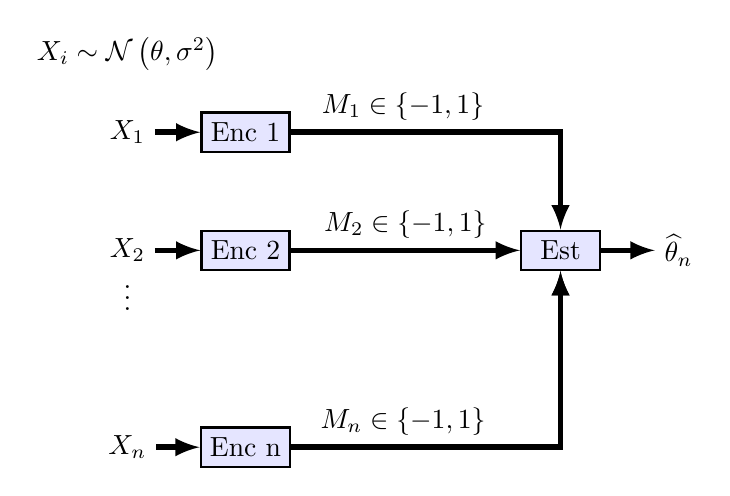
\begin{tikzpicture}[node distance=2cm,auto,>=latex]
  \node at (0,0) (source) {$X_1$} ;
  \node[int1, right of = source, node distance = 1.5cm] (enc1) {Enc 1};  
\draw[->,line width = 2pt] (source) -- (enc1); 

 \node[below of = source, node distance = 1.5cm] (source2) {$X_2$};
\node[int1, right of = source2, node distance = 1.5cm] (enc2) {Enc 2};  
\draw[->,line width = 2pt] (source2) -- (enc2); 

\node[below of = source2, node distance = 2.5cm] (source3) {$X_n$};
\node[int1, right of = source3, node distance = 1.5cm] (enc3) {Enc n};  
\draw[->,line width = 2pt] (source3) -- (enc3); 

\node[above of = source, node distance = 1cm] (dist) {$X_i \sim {\mathcal N} \left(\theta, \sigma^2 \right)$};
\node[below of = source2, node distance = 0.5cm] {$\vdots$};

\node[int1, right of = enc2, node distance = 4cm ] (est) {Est};
\draw[->,line width = 2pt] (enc1) -| node[above, xshift = -2cm] (mes1) {$M_1 \in \left\{-1,1\right\}$} (est);   
\draw[->,line width = 2pt] (enc2) -- node[above, xshift = 0cm] (mes2) {$M_2 \in \left\{-1,1\right\}$} (est);   

\draw[->,line width = 2pt] (enc3) -| (est);   

\draw[->,line width = 2pt] (enc3) -| node[above, xshift = -2cm]  {$M_n \in \left\{-1,1\right\}$} (est);   

\node[right of = est, node distance = 1.5cm] (dest) {$\widehat{\theta}_n$};
%         \node [int1] (dec) [right of=dest, node distance = 1.5cm,  align=center] {\small Dec };
%\node [int1] (enc) [right of = dec, node distance = 3cm]{Enc}; 
%\draw[->,line width=2pt] (dec) -- (dest);
\draw[->, line width=2pt] (est) -- (dest);
\end{tikzpicture}
\end{center}
\caption{\label{fig:sequential} Distributed single-bit encoding.}
\end{figure}


Consider the distributed 1-bit estimation setting of Fig.~\ref{fig:sequential} where $X_n = Z_n + \theta$ with $Z_n$ zero mean and variance $\sigma^2$. Upon observing the $n$th sample $X_n$, the estimator is observing $M_n(X_n) \in \{0,1\}$, where the mapping $M_n : \mathbb R \rightarrow \{0,1\}$ are determined offline in a manner that will be explained below. Denote $A_n = M_n^{-1}(1)$ and set 
\[
U_n = \begin{cases} 1, & \theta \in A_n \\
-1, & \theta \notin A_n. 
\end{cases}
\]
So the $U_n$s are binary random variables that depends only on the initial draw of $\theta$ and the \emph{detection intervals} $A_1,\ldots,A_n$. We define an \emph{error} event $\mathcal E_n$ at the $n$th observation if $U_n \neq M_n(X_n)$, i.e., an error occurs if $\theta \in A_n$ but $\theta + Z_n \notin A_n$ or $\theta \notin A_n$ but $\theta +Z_n \in A_n$. With this notation, the $n$ observation can be seen as the result of noisy transmission of  $U_n$ through a binary channel with bit flip probability of $\mathbb P( \mathcal E_n)$. We now choose the detection regions $A_n$ as follows: we divide the real line into $m = \lfloor   \sqrt{n} /  (\sigma \alpha_n) \rfloor$ equiprobable disjoint intervals $I_1,\ldots,I_m$. For $j=1,\ldots,m$, include $I_j$ in $A_n$ with probability $1/2$. As a result, we can think of the index of the interval where $\theta$ falls as the \emph{message} (one of possible $m$) that is communicated by $n$ uses of the channel from $U_n$ to $M_n(X_n)$. The width of each interval is $\sigma \alpha_n/ \sqrt{n}$, so if this messages is communicated with zero error, we attain an estimate $\widehat{\theta}$ of accuracy 
\[
\left| \theta - \widehat{\theta} \right|  <  \sigma \frac{\alpha_n}{\sqrt{n}}. 
\]

We now derive conditions of $\alpha_n$ such that communication with vanishing probability of error is possible. Note that by the codeword construction we have
\[
\mathbb P(M_n(X_n)=1) = 1/2,
\]
and, assuming $n$ is large enough,
\[
\mathbb P(\mathcal E_n) = \sum_{j=1}^m \mathbb P(\theta \in I_j)  \mathbb P(X_n \notin I_j) /2 \approx 0.5 \mathbb P( |Z_n|> \sigma \alpha_n/\sqrt{n}) \approx 0.5 -  \frac{1}{\sqrt{2\pi}} \frac{\alpha_n}{\sqrt{n}}+O(1/n).
\]
If $\alpha_n / n \rightarrow 0$, then the probability of bitflip goes to $0.5$ as $n$ increases. By the channel coding theorem we know that communication with vanishing probability is possible provided the communication rate
\[
R = \log_2(m) = \log_2(\sqrt{n} / (\sigma \alpha_n)) 
\]
does not exceeds the capacity:
\[
 C = n(1-h( \mathbb P(\mathcal E))) \approx \frac{n}{2\pi \ln 2} \frac{\alpha_n^2}{n} .
\]
The last condition is satisfied provided 
\[
\alpha_n > \sqrt{2 \pi \ln 2 \log_2(\sqrt{n}/\sigma)}.
\]

{\color{red}
Use Fano's inequality to prove a necessary condition on $\alphan_n$ and therefore on asymptotic relative efficiency.
}

 
%We use
%\[
%\Phi(x) = 0.5  + \frac{1}{\sqrt{2 \pi} }e^{-x^2/2} \left[x+\frac{x^3}{3}+... \right] 
%\]
%\[
%h(0.5 - x) = 1- \frac{1}{2 \ln 2} \sum_{n=1}^\infty  \frac{2^{2n} x^{2n}} {n(2n-1)}
%\]

%%%%%%%%%%%%%%%%%%%%%%%%%%%%%%%%%%%%%%%%%%%%%%%%%%%%%%%%%%%%%%%%%%%%%%%%%%%%%%%%
\bibliographystyle{IEEEtran}
\bibliography{IEEEabrv,/Users/Alon1/LaTex/bibtex/sampling}


\end{document}
